\subsection{Simulator}

Das Erarbeiten des Konzeptes des Simulators, der Implementierung und des Gebrauchs wird in diesem Kapitel festgehalten.

Nach der Nutzwertanalyse war das grundlegende Konzept klar und es konnte mit der Implementierung begonnen werden.

\subsubsection{Spezifikationen}

TODO: Was soll Simulator koennen?

\begin{table}[H]
\centering
\small
\begin{tabularx}{\textwidth}{|l|X|l|}
\hline
  \textbf{Nr.} & \textbf{Spezifikation} & \textbf{Priorität 1-3}  \\
  \hline
  1  & Der Zielknoten kann ausgewählt werden. &  2\\
  \hline
   2   & Der Roboter speichert den Graph intern.  & 1\\
  \hline
   3 & Der Roboter überprüft seine Nachbarsknoten.&1\\
  \hline
  4 & Der Roboter erkennt fehlende Linien und reagiert darauf. & 1\\
  \hline
  5 &   Der Roboter erkennt Pylonen und reagiert darauf. & 1\\
  \hline
   6  &   Der Roboter erkennt Barrieren und reagiert darauf. & 1\\
  \hline
    7 &   Der Roboter berechnet den kürzesten Weg im Graphen.& 1\\
  \hline
     8  &   Der Weg des Roboters wird im GUI angezeigt. & 1\\
  \hline
      9   &   Die Reaktionen auf die Hindernisse werden im GUI angezeigt. & 2\\
  \hline
 10   &   Die Hindernisse werden im GUI angezeigt. & 2\\
  \hline
   11   &   Die Reihenfolge der Knoten wird erkannt, als Vorbereitung, dass der Roboter, der Steuerung sagen kann, wo sich der nächste Weg befindet. & 3\\
  \hline

\end{tabularx}
\caption{Spezifikationen Simulator}
\label{table:spezifikation-simulator}
\end{table}

\subsubsection{Konzeption}

Es wurden mehrere Varianten ermittelt mit einem morphologischen Kasten, die alle die Spezifikatinen erfuellen koennen. Mit einer Nutzwertanalyse wurde die beste Variante bestimmt.

TODO BEschreib gewaehlte Variante, depending wo Kasten \& Analyse sind in Doku

Die einzelnen Taetigkeiten wurden in GitHub Issues festgehalten. Jedes Issue wurde jeweils der Person zugeordnet, die gerade daran arbeitet. So konnte koordiniert entwickelt werden.

\begin{figure}[H]
\centering
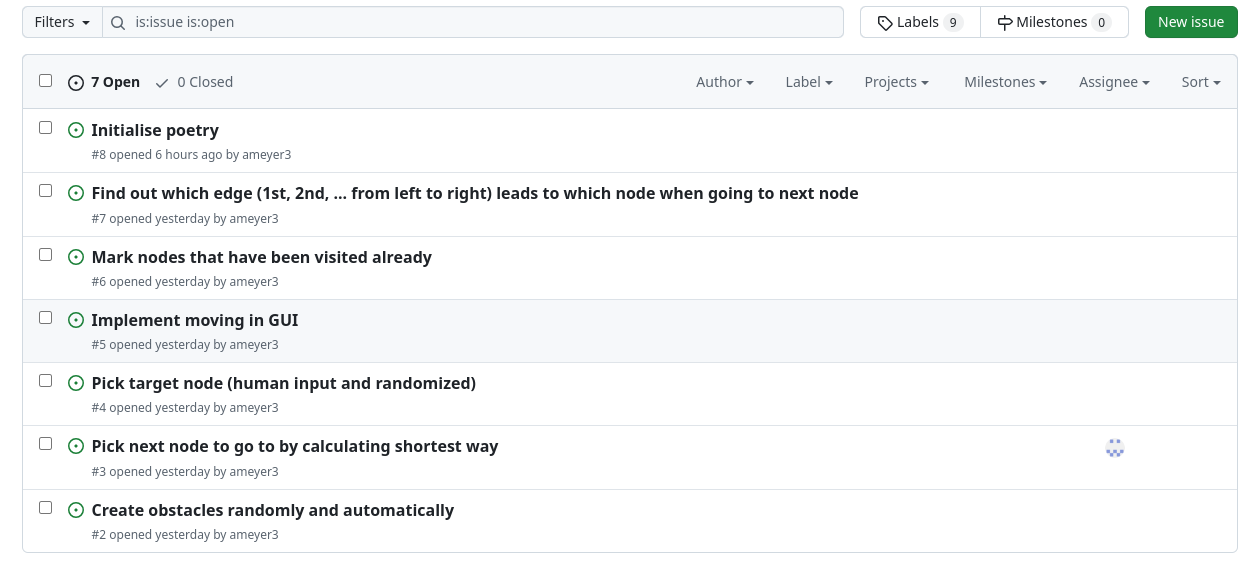
\includegraphics[width=\textwidth]{img/github-issues.png}
\caption{GitHub Issue Liste}
\label{fig:github-issues}
\end{figure}

Es wurde ein objektorientierter Ansatz gewaehlt, um den Simulator umzusetzen. Die Roboterklasse soll dabei den physischen Roboter darstellen, der die einzelnen Bauteile besitzt. So soll zum Beispiel die Wheels Klasse verwendet werden als Simulation fuer das Drehen und fortbewegen. An dieser Klasse werden diese Nachrichten gesendet, die im echten Roboter an die elektrische Steuerung gesendet werden wuerden betreffend der Fortbewegung.


\begin{figure}[H]
\centering
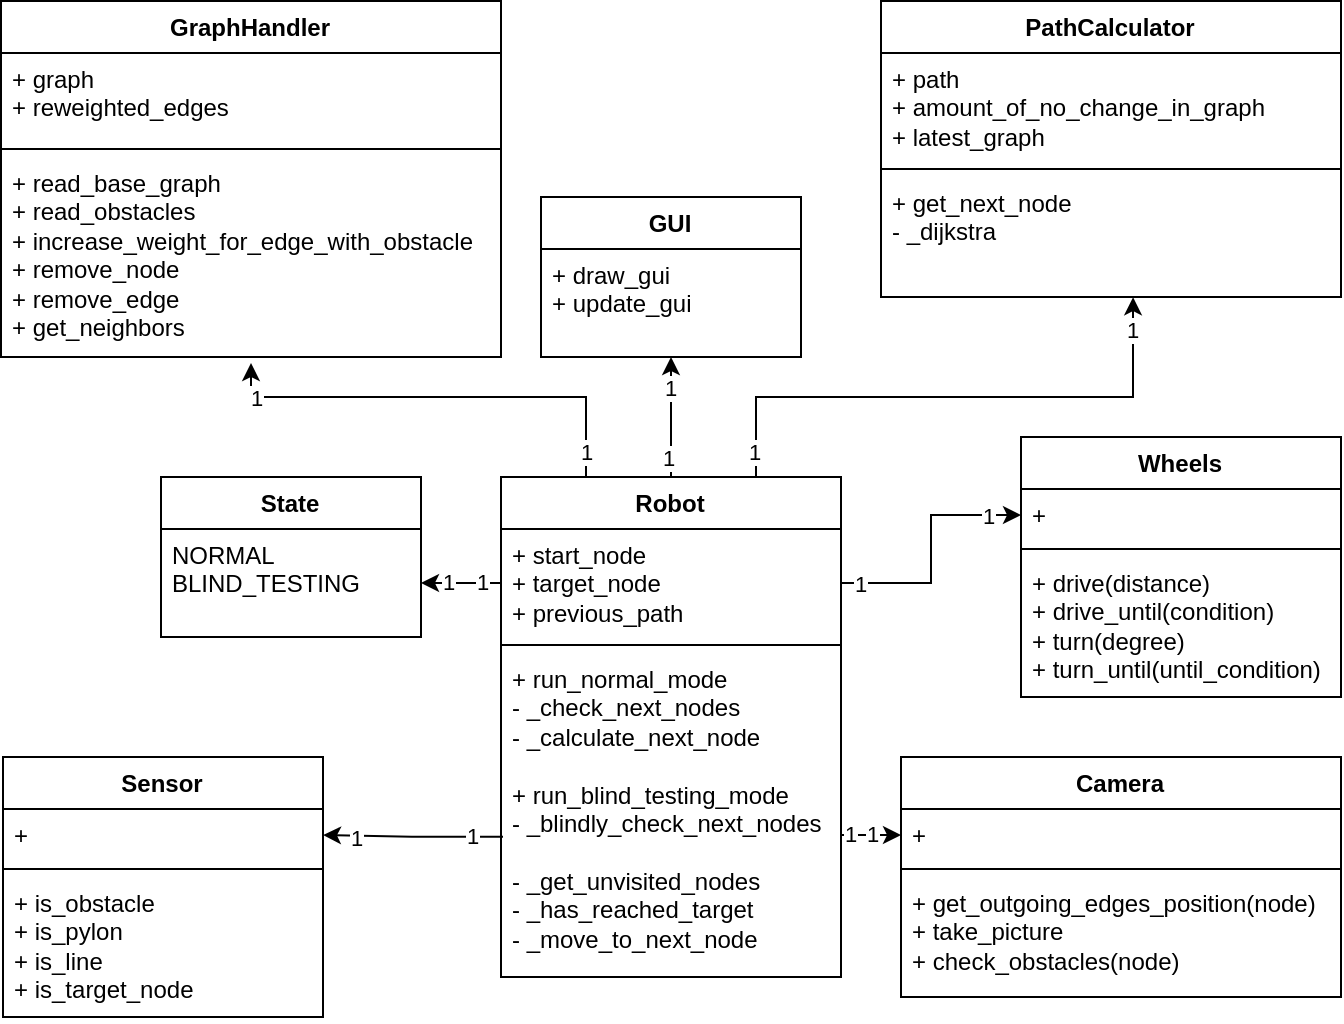
\includegraphics[width=\textwidth]{assets/informatik-prototyp/simulator/simulator-erd.png}
\caption{Simulator ERD}
\label{fig:simulator-erd}
\end{figure}

\subsubsection{Entwicklung}

Der erste Schritt war es einen Graph zu definieren. Dazu wurde ein YAML File mit dem konfigurierten Graph erstellt. 
Dazu wurde der vorgegebene Graph beschriftet: Jeder Knoten erhaelt einen Buchstaben und jede Kante ein Gewicht. Die Gewichtungen sind die relativen Laengen der Strecken. Diese Beschriftung wurde wie folgt in einem YAML File beschrieben.

\begin{figure}[H]
\begin{subfigure}{0.275\textwidth}
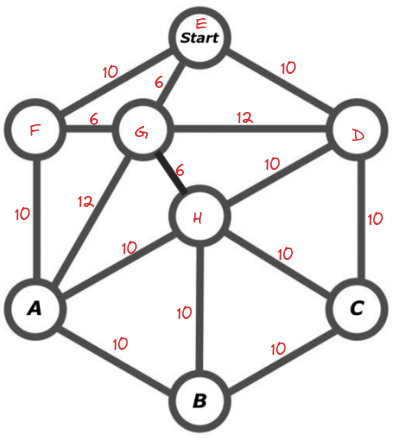
\includegraphics[width=0.95\linewidth]{img/graph_with_weighted_edges.png} 
\caption{Beschrifteter Graph}
\label{fig:labeled-graph}
\end{subfigure}
\begin{subfigure}{0.720\textwidth}
\begin{footnotesize}
\begin{verbatim}
# the edges are assorted clock-wise
A: [{ F: 10 }, { G: 12 }, { H: 10 }, { B: 10 }]
B: [{ A: 10 }, { H: 10 }, { C: 10 }]
C: [{ D: 10 }, { B: 10 }, { H: 10 }]
D: [{ E: 10 }, { C: 10 }, { H: 10 }, { G: 12 }]
E: [{ D: 10 }, { G: 6 }, { F: 10 }]
F: [{ E: 10 }, { G: 6 }, { A: 10 }]
G: [{ E: 6 }, { D: 12 }, { H: 6 }, { A: 12 }, { F: 6 }]
H: [{ G: 6 }, { D: 10 }, { C: 10 }, { B: 10 }, { A: 10 }]
\end{verbatim}
\end{footnotesize}
\caption{Graph in YAML}
\label{fig:graph-yaml}
\end{subfigure}
\end{figure}

Die Hindernisse und die fehlenden Linien sind ebenfalls in einem YAML File definiert. So koennen diese einfach angepasst werden:

\begin{verbatim}
cone:
  - F
barrier:
  - [E, G]
missing_line:
  - [E, D]
\end{verbatim}

Der 
- Roboter liest Graph, ueberprueft Nodes und Barrieren
-> add Graph YAML \& Barriere YAML

- Calculator holt kürzester Weg, Roboter geht zu nächsten Node

- Poetry

- Die einzelnen Kanten werden identifiziert mit Sortierung

- GUI Roboter bewegt sich

- GUI Hindernisse aufgezeigt in GUI

- Trial and error mode; Knoten verloren